\documentclass[a4paper,
fontsize=11pt,
%headings=small,
oneside,
numbers=noperiodatend,
parskip=half-,
bibliography=totoc,
final
]{scrartcl}

\usepackage[babel]{csquotes}
\usepackage{synttree}
\usepackage{graphicx}
\setkeys{Gin}{width=.7\textwidth} %default pics size

\graphicspath{{./plots/}}
\usepackage[ngerman]{babel}
\usepackage[T1]{fontenc}
%\usepackage{amsmath}
\usepackage[utf8x]{inputenc}
\usepackage [hyphens]{url}
\usepackage{booktabs} 
\usepackage[left=2.4cm,right=2.4cm,top=2.3cm,bottom=2cm,includeheadfoot]{geometry}
\usepackage{eurosym}
\usepackage{multirow}
\usepackage[ngerman]{varioref}
\setcapindent{1em}
\renewcommand{\labelitemi}{--}
\usepackage{paralist}
\usepackage{pdfpages}
\usepackage{lscape}
\usepackage{float}
\usepackage{acronym}
\usepackage{eurosym}
\usepackage{longtable,lscape}
\usepackage{mathpazo}
\usepackage[normalem]{ulem} %emphasize weiterhin kursiv
\usepackage[flushmargin,ragged]{footmisc} % left align footnote
\usepackage{ccicons} 
\setcapindent{0pt} % no indentation in captions

%%%% fancy LIBREAS URL color 
\usepackage{xcolor}
\definecolor{libreas}{RGB}{112,0,0}

\usepackage{listings}

\urlstyle{same}  % don't use monospace font for urls

\usepackage[fleqn]{amsmath}

%adjust fontsize for part

\usepackage{sectsty}
\partfont{\large}

%Das BibTeX-Zeichen mit \BibTeX setzen:
\def\symbol#1{\char #1\relax}
\def\bsl{{\tt\symbol{'134}}}
\def\BibTeX{{\rm B\kern-.05em{\sc i\kern-.025em b}\kern-.08em
    T\kern-.1667em\lower.7ex\hbox{E}\kern-.125emX}}

\usepackage{fancyhdr}
\fancyhf{}
\pagestyle{fancyplain}
\fancyhead[R]{\thepage}

% make sure bookmarks are created eventough sections are not numbered!
% uncommend if sections are numbered (bookmarks created by default)
\makeatletter
\renewcommand\@seccntformat[1]{}
\makeatother

% typo setup
\clubpenalty = 10000
\widowpenalty = 10000
\displaywidowpenalty = 10000

\usepackage{hyperxmp}
\usepackage[colorlinks, linkcolor=black,citecolor=black, urlcolor=libreas,
breaklinks= true,bookmarks=true,bookmarksopen=true]{hyperref}
\usepackage{breakurl}

%meta

%meta

\fancyhead[L]{A. Bertino, J. Rohden \\ %author
LIBREAS. Library Ideas, 36 (2019). % journal, issue, volume.
\href{http://nbn-resolving.de/}
{}} % urn 
% recommended use
%\href{http://nbn-resolving.de/}{\color{black}{urn:nbn:de...}}
\fancyhead[R]{\thepage} %page number
\fancyfoot[L] {\ccLogo \ccAttribution\ \href{https://creativecommons.org/licenses/by/4.0/}{\color{black}Creative Commons BY 4.0}}  %licence
\fancyfoot[R] {ISSN: 1860-7950}

\title{\LARGE{Support, Bedarfserhebung, Wissensvermittlung: Der DARIAH-DE Helpdesk}} % title
\author{Andrea Bertino, Jan Rohden} % author

\setcounter{page}{1}

\hypersetup{%
      pdftitle={Support, Bedarfserhebung, Wissensvermittlung: Der DARIAH-DE Helpdesk},
      pdfauthor={Andrea Bertino, Jan Rohden},
      pdfcopyright={CC BY 4.0 International},
      pdfsubject={LIBREAS. Library Ideas, 36 (2019).},
      pdfkeywords={Bibliothek, Open Access, Nachhaltigkeit, Support, Organisationsstruktur, Forschungsinfrastruktur},
      pdflicenseurl={https://creativecommons.org/licenses/by/4.0/},
      pdfcontacturl={http://libreas.eu},
      baseurl={http://libreas.eu},
      pdflang={de},
      pdfmetalang={de}
     }



\date{}
\begin{document}

\maketitle
\thispagestyle{fancyplain} 

%abstracts
\begin{abstract}
\noindent
\textbf{Kurzfassung}: Die Nachhaltigkeit einer digitalen
Forschungsinfrastruktur hängt nicht nur von Technik, sondern vor allem
von dem Vertrauen ihrer NutzerInnen ab. Dieses Vertrauen wiederum
resultiert insbesondere aus dem erkennbaren Mehrwert, den die Angebote
der Forschungsinfrastruktur den NutzerInnen bieten können. Um diesen
Mehrwert dauerhaft bieten zu können, müssen die Dienste einer Virtuellen
Infrastruktur nicht nur kontinuierlich weiterentwickelt werden, sondern
es ist auch notwendig, dass die NutzerInnen bei allen mit der Verwendung
der Angebote verbundenen Fragen unterstützt werden. Der vorliegende
Beitrag skizziert ein Modell, um fortlaufende Weiterentwicklung und
nutzerfreundliche Unterstützungsangebote der Infrastruktur zu vereinen.
Die Grundlage dafür bildet eine Neubetrachtung des Helpdesks von
DARIAH-DE, der deutschen Beteiligung an der europäischen
Forschungsinfrastruktur DARIAH-EU (Digital Research Infrastructure for
the Arts and Humanities).

\begin{center}\rule{0.5\linewidth}{\linethickness}\end{center}

\textbf{Abstract}: The sustainability of a digital research
infrastructure relies not only on technology, but first and foremost on
the trust of its users. In turn, this trust results in particular from
the tangible added value that the services provided by the research
infrastructure offer its users. In order to be able to offer this added
value on an ongoing basis, the services of a virtual research
infrastructure must not only be continuously developed, but it is also
necessary that the users are supported in all questions regarding the
use of the services. This article outlines a model for integrating
continuous development and user-friendly infrastructure support
services. The basis for this outline is a reassessment of the helpdesk
of DARIAH-DE, Germany's participation in the European research
infrastructure DARIAH-EU (Digital Research Infrastructure for the Arts
and Humanities).
\end{abstract}

%body
\hypertarget{nachhaltigkeit-und-digitale-infrastrukturen}{%
\section{Nachhaltigkeit und digitale
Infrastrukturen}\label{nachhaltigkeit-und-digitale-infrastrukturen}}

Nachhaltigkeit ist in den vergangenen Jahren zu einem wichtigen Thema im
politischen Diskurs geworden: ob in Bezug auf die Energiewende, das
Recycling oder das Wirtschaftssystem: Nachhaltigkeit wird stets als
erstrebenswertes Ideal deklariert.\footnote{Vergleiche zur
  Nachhaltigkeit umfassend Pufé, I. (2017). Nachhaltigkeit. 3.,
  überarbeitete und erweiterte Auflage. Konstanz/München: UVK (utb,
  8705).} Im wissenschaftspolitischen Diskurs ist dieser Trend ebenfalls
zunehmend zu erkennen, auch wenn hierbei der Begriff der Nachhaltigkeit
ein wenig anders akzentuiert wird: Neben der Nachhaltigkeit von
Ressourcen oder Technik wird im wissenschaftspolitischen Kontext in
stärkerem Maße die Nachhaltigkeit von Betriebsmodellen thematisiert. Im
Zuge dessen wird das Konzept der Nachhaltigkeit somit über materielle
Güter hinaus auf immaterielle Modelle und Strukturen ausgeweitet. Ein
Paradebeispiel hierfür sind digitale Infrastrukturen, die häufig
spezialisierte technische Systeme und elaborierte Organisations- und
Wissensstrukturen in sich vereinen. Wenn digitale Infrastrukturen
Nachhaltigkeit anstreben, so stehen sie damit vor der Herausforderung,
dies in gleich zweifacher Hinsicht gewährleisten zu müssen, einerseits
in Bezug auf die Technik,\footnote{Vergleiche hierzu Gietz, P. \&
  Hütter, H. (2016). Der Aufbau einer nachhaltigen technischen
  Infrastruktur für die Geisteswissenschaften: Die DARIAH-DE eHumanities
  Infrastructure Service Unit (DeISU). \emph{Bibliothek Forschung und
  Praxis}, 40(2), pp. 244-249.
  \url{https://doi.org/10.1515/bfp-2016-0029}.} andererseits im Hinblick
auf das mit ihnen verbundene spezialisierte Wissen sowie dessen
Organisation. Beide Aspekte sind nicht zuletzt deshalb untrennbar
miteinander verknüpft, weil digitale Infrastrukturen in besonders
starkem Maße auf ihre Zielgruppe angewiesen sind: die
NutzerInnen.\footnote{Vergleiche zur Nachhaltigkeit digitaler
  Infrastrukturen auch Blümm, M., Neuroth, H. \& Schmunk, S. (2016).
  DARIAH-DE -- Architecture of Participation. \emph{Bibliothek Forschung
  und Praxis}, 40(2), pp.~165-171.
  \url{https://doi.org/10.1515/bfp-2016-0026}.} NutzerInnen greifen
jedoch nur dann auf Virtuelle Infrastrukturen zurück, wenn sie Vertrauen
in die Infrastruktur selbst und in die im Rahmen dessen angebotenen
Dienste setzen. Jenes Vertrauen gewinnen digitale Infrastrukturen vor
allem dadurch, dass sie für NutzerInnen einen erkennbaren Mehrwert
bieten. Dafür müssen sie vier Anforderungen erfüllen:

\begin{enumerate}
\def\labelenumi{\arabic{enumi}.}
\item
  Eine digitale Infrastruktur muss Angebote mit niederschwelligem Zugang
  bereitstellen, die sich für verschiedene Einsatzzwecke eignen.
\item
  Für jedes Angebot muss die Infrastruktur Supportdienste bieten, die
  NutzerInnen bei dessen Verwendung oder bei Fragen unterstützen.
\item
  Die Angebote der Infrastruktur müssen an den Bedarfen der Nutzenden
  ausgerichtet und fortlaufend weiterentwickelt werden. Dafür ist
  spezialisiertes ExpertInnenwissen erforderlich, das nicht nur
  nachhaltig gesichert, sondern zudem stets aktualisiert und damit
  erweitert werden muss.
\item
  Das aus der Entwicklung der Infrastruktur gewonnene Erfahrungswissen
  sollte den NutzerInnen verfügbar gemacht werden, möglichst in
  Anknüpfung an deren Einsatzszenarien.
\end{enumerate}

Für eine nachhaltige Entwicklung von Virtuellen Infrastrukturen ist es
wichtig, jene vier Aspekte nicht isoliert zu betrachten, sondern in Form
eines kontinuierlichen Entwicklungsprozesses miteinander zu verbinden.

Ziel des vorliegenden Beitrags ist es, ausgehend von der Virtuellen
Forschungsinfrastruktur für die Geistes- und Kulturwissenschaften
DARIAH-DE\footnote{\url{https://de.dariah.eu/startseite} (11.10.19).}
ein Modell für die nachhaltige Entwicklung von Infrastrukturen zu
skizzieren, das auf zwei Bausteinen basiert: Einerseits auf dem
beständigen und systematischen Austausch mit der Community, andererseits
auf der proaktiven Vermittlung von Informationen an die NutzerInnen.
Eine zentrale Rolle für die Vermittlung dieser beiden Aspekte spielt,
wie dargelegt werden soll, der Helpdesk.

\hypertarget{dariah-de-clarin-d-clariah-de}{%
\section{DARIAH-DE + CLARIN-D =
CLARIAH-DE}\label{dariah-de-clarin-d-clariah-de}}

DARIAH-DE ist eine Forschungsinfrastruktur für die digital arbeitenden
Geistes- und Kulturwissenschaften. Sie besteht aus einer Kooperation
deutscher Partnerinstitutionen, die den deutschen Beitrag zu dem
europäischen Netzwerk DARIAH-EU bilden.\footnote{Die Digitale
  Forschungsinfrastruktur für die Geistes- und Kulturwissenschaften
  (DARIAH) hat zum Ziel, die digital gestützte Forschung und Lehre in
  allen Geistes- und Kulturwissenschaften zu verbessern und zu fördern.
  DARIAH entwickelt, unterhält und betreibt eine Infrastruktur zur
  Unterstützung ICT-gestützter Forschungspraktiken und unterstützt
  Forscher dabei, diese für den Aufbau, die Analyse und die
  Interpretation digitaler Ressourcen zu nutzen. DARIAH-EU wurde im
  August 2014 als European Research Infrastructure Consortium (ERIC)
  gegründet. Derzeit hat DARIAH-EU 18 Mitglieder und mehrere
  Kooperationspartner in acht Drittländern. \url{https://www.dariah.eu/}
  (11.10.19).} Nach den ersten drei durch das Bundesministerium für
Bildung und Forschung (BMBF) geförderten Phasen, die vor allem auf den
Aufbau der Infrastruktur und die Konsolidierung ihrer Governancestruktur
abzielten, befindet sich DARIAH-DE seit März 2019 in einer sogenannten
\enquote{Betriebskooperation}.\footnote{\url{https://de.dariah.eu/der-forschungsverbund}
  (11.10.19).} Im Rahmen dessen haben sich 16 Partnerinstitutionen auf
den nachhaltigen Betrieb und die Verstetigung der im Zuge von DARIAH-DE
entwickelten Angebote verständigt. Bis zum Ende der Betriebskooperation
im Februar 2021 wird DARIAH-DE sein Angebotsportfolio mit den Angeboten
von CLARIN-D\footnote{CLARIN-D zielt auf den Aufbau eines mit
  ausgewählten Fachdisziplinen eng verbundenen Zentrenverbunds als
  Rückgrat einer Forschungsinfrastruktur insbesondere für
  WissenschaftlerInnen in den Geistes- und Sozialwissenschaften ab. Die
  Disziplinen decken ein breites Spektrum der Geisteswissenschaften ab,
  für die Sprachressourcen eine zentrale Rolle in der Forschung spielen.
  \url{https://www.clarin-d.net/de/} (11.10.19).} zusammenführen und auf
diese Weise die Vernetzung der digital forschenden Geistes- und
Kulturwissenschaften auf nationaler und europäischer Ebene weiter
vorantreiben. Zu diesem Zweck fördert das BMBF seit März 2019 das
Projekt CLARIAH-DE.\footnote{\url{http://www.clariah.de/} (11.10.19).}

\begin{figure}
\centering
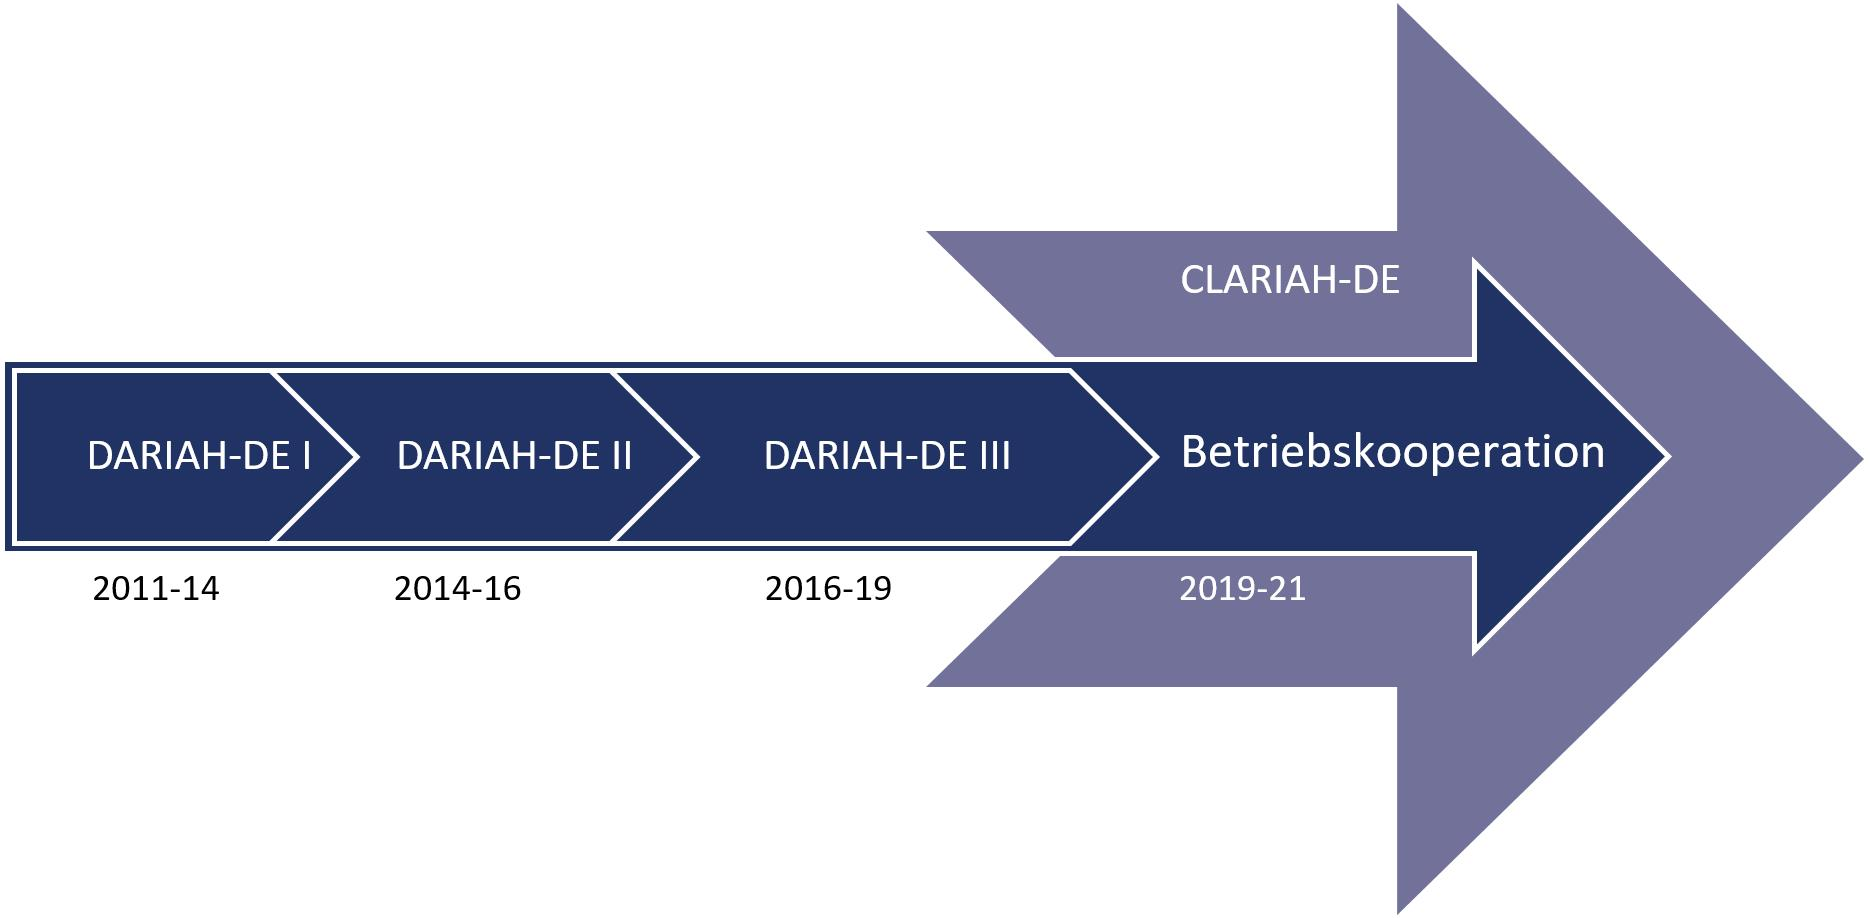
\includegraphics{img/DARIAHEntwicklung.jpg}
\caption{DARIAH-DE Entwicklung (Bild: Jan Rohden, CC BY-SA 4.0)}
\end{figure}

CLARIN-D und DARIAH-DE haben über die Jahre ein breites Spektrum an
unterschiedlichen Angeboten aufgebaut.\footnote{\url{https://de.dariah.eu/list-services}
  (11.10.19).} Deren Entwicklung erfolgte im beständigen Austausch mit
den unterschiedlichen Fachcommunitys und orientierte sich an deren
Bedarfen.\footnote{Hierzu dienten unter anderem diverse Veranstaltungen.
  Vergleiche \url{https://de.dariah.eu/veranstaltungen} (11.10.19) sowie
  Busch, A., Meister, J. \& Schumacher, M. (2016). Wo bleibt eigentlich
  der einzelne Fachwissenschaftler? \emph{Bibliothek Forschung und
  Praxis}, 40(2), pp.~278-282.
  \url{https://doi.org/10.1515/bfp-2016-0028}.} Die Webportale von
CLARIN-D und DARIAH-DE fungieren jeweils als Einstiegsplattformen,
welche die Angebote präsentieren und einen Zugang dazu gewähren.

Die Zusammenführung der beiden Virtuellen Forschungsinfrastrukturen zu
CLARIAH-DE hat zwei Konsequenzen für die Struktur und Präsentation der
jeweiligen Angebote: Zum einen entsteht dadurch ein neues, noch
vielfältigeres Spektrum an Diensten. Zum anderen führt die
Zusammenführung von CLARIN-D und DARIAH-DE auch zu einer Verschmelzung
von zwei bislang unterschiedlichen Communitys. Dadurch geraten
ursprünglich an den Anforderungen einer einschlägigen NutzerInnenschaft
entwickelte Angebote in stärkerem Maße als zuvor in das Blickfeld
anderer NutzerInnengruppen. Dies kann dazu führen, dass die bisherige
Präsentation der Angebote ebenso wie der jeweilige Zugang dazu mit Blick
auf die Anforderungen neuer Gruppen weiterentwickelt werden muss.

Ein Ansatz dafür ist die Etablierung einer zentralen Anlauf- und
Koordinationsstelle. Eine solche ist sowohl für die NutzerInnen von
Vorteil, als auch für die Infrastruktur selbst: Für NutzerInnen bieten
eine solche Koordinationsstelle die Möglichkeit, bei Nachfragen,
Problemen und für Anregungen mit sachkundigen AnsprechpartnerInnen in
Kontakt treten zu können, ohne selbst die jeweiligen ExpertInnen
ausfindig machen zu müssen. Die Infrastruktur hingegen erhält auf diese
Weise an realen Nutzungsszenarien orientierte Rückmeldungen zu den
eigenen Angeboten und damit wertvolle Informationen für die
Weiterentwicklung der eigenen Dienste. Diese können unter anderem
Fehler, Lücken oder Entwicklungsmöglichkeiten betreffen, aber womöglich
auch auf mangelnde Zugänge oder eine ungeeignete Präsentation für
einzelne Zielgruppen aufmerksam machen.

Um einen Mehrwert für NutzerInnen und Infrastruktur gleichermaßen bieten
zu können, muss eine Koordinationsstelle vier Anforderungen erfüllen:

\begin{enumerate}
\def\labelenumi{\arabic{enumi}.}
\item
  Sie muss ein beständiges Team aus festen AnsprechpartnerInnen
  umfassen;
\item
  es müssen klare Kommunikationskanäle zu Kontaktpersonen für die
  einzelnen Angebote bestehen, die in kurzer Zeit zu erreichen sind;
\item
  jede Anfrage muss inklusive dem dazugehörigen Kommunikations- und
  Lösungsprozess lückenlos an einer zentralen Stelle dokumentiert
  werden;
\item
  Anfragen sollten kategorisierbar und in ihrer Gesamtheit statistisch
  auswertbar sein, um aktuelle Trends und Entwicklungen erkennbar zu
  machen.
\end{enumerate}

\hypertarget{der-dariah-de-helpdesk}{%
\section{Der DARIAH-DE Helpdesk}\label{der-dariah-de-helpdesk}}

Zur effizienten Organisation und Beantwortung von NutzerInnenanfragen
wurde für DARIAH-DE ein über das Webportal erreichbarer Helpdesk
eingerichtet, der technisch auf dem Ticketsystem der
Open-Source-Software OTRS basiert. In OTRS ist es möglich, eine Struktur
verschiedener \enquote{Queues}, also Warteschlangen beziehungsweise
Gruppen anzulegen, in die eingehende Anfragen (sogenannte Tickets)
eingeordnet werden können.\footnote{Im Falle von DARIAH-DE erfolgt die
  erste Einordnung von Tickets in die einzelnen Queues derzeit durch
  Hilfskräfte des DARIAH-DE Betriebspartners DAASI International. Bei
  nicht eindeutigen Fällen oder Unklarheiten konsultieren die
  Hilfskräfte das DARIAH-DE Coordination Office, dem die Koordination
  der DARIAH-DE Betriebskooperation obliegt.} Jeder dieser Queues kann
MitarbeiterInnen zugeordnet werden, die bei Eingang eines Tickets
automatisch benachrichtigt werden. Stellt sich heraus, dass ein Ticket
in einen anderen Zuständigkeitsbereich fällt, kann das betreffende
Ticket entweder in eine andere Queue verschoben oder MitarbeiterInnen
persönlich zugewiesen werden. Das System ermöglicht natürlich auch die
Kontaktaufnahme mit dem Urheber der Anfrage. Alle jene Prozesse von der
Erstellung bis zum Schließen des Tickets werden vom System dokumentiert.
Auf diese Weise erlaubt OTRS es, den mit einer Anfrage verbundenen
Bearbeitungs- und Kommunikationsprozess im Team zu koordinieren und
dafür zu sorgen, dass Anfragen die zuständigen AnsprechpartnerInnen
erreichen. Es ermöglicht dadurch einen effizienten First Level Support.

Mit der Einrichtung seines Helpdesks etablierte DARIAH-DE darüber hinaus
eine organisatorische Struktur, um Anfragen innerhalb einer vertretbaren
Reaktionszeit beantworten zu können. Wichtig dafür war zunächst der
Aufbau eines Support-Teams zur Betreuung des Helpdesks. Dieses umfasst
GeisteswissenschaftlerInnen, InformatikerInnen,
InformationswissenschaftlerInnen und BibliothekarInnen. Das Team
beinhaltet somit sowohl mit geistes- und kulturwissenschaftlichen
Forschungsprozessen vertraute Mitglieder als auch MitarbeiterInnen mit
Kompetenzen in den Bereichen Technik und Informationsverarbeitung.

Im Rahmen der Zusammenführung von CLARIN-D und DARIAH-DE zu CLARIAH-DE
werden auch die Helpdesks beider Infrastrukturen zusammengefasst. Dies
erfordert die Anpassung der Organisationsstruktur der Helpdesks an das
zukünftig vielfältigere Angebotsportfolio. Die vorausschauende
Gestaltung der neuen Queues ist dabei von zentraler Bedeutung: diese
muss sicherstellen, dass die jeweils zuständigen Teammitglieder
möglichst umgehend auf ihren Zuständigkeitsbereich betreffende Tickets
hingewiesen werden, um eine Antwort innerhalb der festgelegten
Reaktionszeit zu ermöglichen. Das DARIAH-DE Coordination Office hat
daher ein Verfahren für die Erstellung jeder neuen Queue festgelegt, das
die Erhebung der folgenden Daten umfasst:

\begin{enumerate}
\def\labelenumi{\arabic{enumi}.}
\item
  Name des Workflows
\item
  Beschreibung des Workflows
\item
  Zuordnung von Verantwortlichen/MitarbeiterInnen zur Bearbeitung der
  Anfragen
\item
  Sinnvolle Textvorlagen (optional)
\item
  Spezielle Signaturen (optional)
\end{enumerate}

Alle diese Informationen werden auf einer einschlägigen Seite im
DARIAH-DE Wiki dokumentiert.

Mit der Anpassung des Helpdesks bieten sich zudem Möglichkeiten zur
Weiterentwicklung der Angebote von CLARIAH-DE. Voraussetzung dafür ist
allerdings, das Ticketsystem nicht nur als bloßes Werkzeug zur
Beantwortung von Anfragen zu begreifen, sondern darüber hinaus als
nützliche Informationsquelle. Anfragen von NutzerInnen sind häufig
jedoch sehr spezifisch und komplex. Daher empfiehlt sich eine stärkere
Verknüpfung zwischen dem First Level Support (dem eigentlichen
Helpdesk), der fortlaufenden Dokumentation des durch die Beratung
erworbenen Fachwissens (Second Level Support) und der Prüfung
potentieller Entwicklungschancen durch ExpertInnen unterschiedlicher
Bereiche (Third Level Support). Auf diese Weise ist es möglich, die aus
Anfragen hervorgehenden Bedarfe stärker als bisher für die
Fortentwicklung der Angebote heranzuziehen. Konkret bedeutet dies:
Fragen sollen nicht nur beantwortet werden, sondern außerdem als
Ausgangspunkt für transparente Informationsangebote dienen, die im
Idealfall verhindern, dass die gleiche Frage erneut gestellt wird.
Anders formuliert: Informationsbedarf soll zu Wissensaufbau und
-präsentation führen.

\begin{figure}
\centering
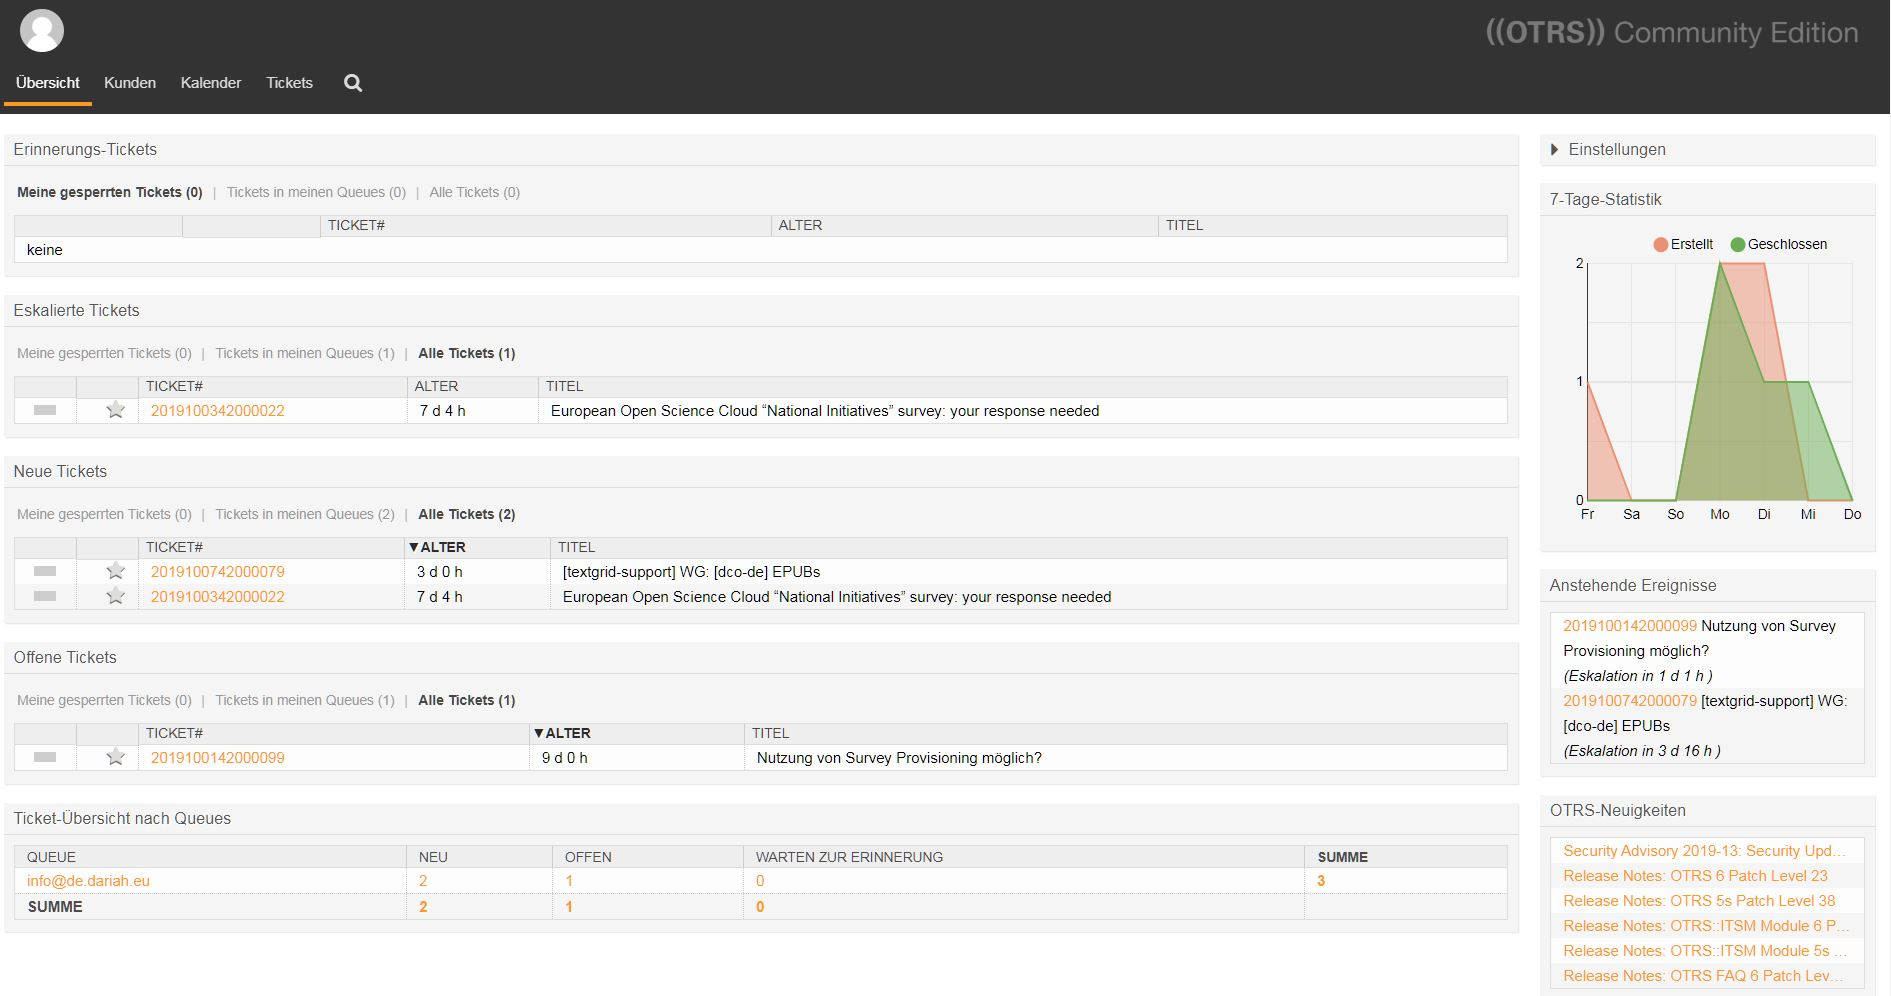
\includegraphics{img/OTRS.jpg}
\caption{OTRS-System des DARIAH-DE Helpdesks (Screenshot: Andrea
Bertino, CC BY-SA 4.0)}
\end{figure}

\hypertarget{personen-oder-queues}{%
\section{Personen oder Queues?}\label{personen-oder-queues}}

Zur Konzeption der zukünftigen Struktur wurden die bisherigen Queues
inklusive der ihnen zugeordneten Tickets analysiert. Dabei stellte sich
zwar einerseits heraus, dass der Helpdesk regelmäßig genutzt wird.
Andererseits zeigte sich ebenfalls, dass NutzerInnen nach Erhalt einer
hilfreichen Antwort auf ihre Anfrage bei späteren Anliegen oftmals
direkt die VertreterInnen des jeweiligen Angebots kontaktierten, ohne
den Helpdesk dafür heranzuziehen. Dieses Vorgehen hat zwar einerseits
den Vorzug, dass NutzerInnen auf diese Weise in den kommunikativen
Austausch mit MitarbeiterInnen der Angebote treten, dadurch Vertrauen
schöpfen und zur Nutzung jener Dienste angeregt werden. Andererseits
resultiert daraus jedoch ein gravierender Nachteil: Die Kommunikation
findet zumeist über persönliche Kommunikationskanäle statt (in der Regel
E-Mail oder Telefon), sodass das aus der Beantwortung der Anfrage
resultierende Erfahrungswissen zwischen NutzerInnen und den
AnsprechpartnerInnen des jeweiligen Angebots verbleibt. Der Austausch
wird somit in der Regel nicht dokumentiert und kann deswegen nicht
nachgenutzt werden. Jeglicher Mehrwert für die Weiterentwicklung des
jeweiligen Angebots geht somit verloren.

Dies wirft eine wichtige Frage für die Betreuung im Allgemeinen auf,
nämlich inwieweit Beratung oder technischer Support überhaupt an
einzelne Personen gebunden sein sollten. Wenn NutzerInnen es vorziehen,
bekannte AnsprechpartnerInnen zu kontaktieren oder Personen, die sie
aufgrund von Vorkenntnissen oder Informationen aus etablierten
Netzwerken als kompetent für ihre Anfrage erachten, so könnte man daraus
die These ableiten, ein Helpdesk sei unnötig. Eine solche Argumentation
lässt jedoch außer Acht, dass \emph{ein Helpdesk einen wichtigen Beitrag
zur Nachhaltigkeit leistet, insbesondere im Hinblick auf Virtuelle
Forschungsinfrastrukturen.} Letztere werden in Deutschland nämlich
häufig im Rahmen projektbezogener Förderung aufgebaut, weswegen die
daran beteiligten MitarbeiterInnen oft befristete Arbeitsverträge
besitzen. Daraus resultiert eine hohe Personalfluktuation, sodass
Referenzkontakte und selbst persönliche Netzwerke in der Regel nicht von
Dauer sind. Neue MitarbeiterInnen hingegen benötigen in der Regel eine
gewisse Einarbeitungszeit, bis sie den Wissensstand der VorgängerIn
erreicht haben. Während dieser Phase kann eine Rückmeldung der erbetenen
Informationen in der üblichen Reaktionszeit nicht immer gewährleistet
werden, was sich negativ auf das Vertrauen der NutzerInnen in die
einzelnen Angebote und in die Infrastruktur im Allgemeinen auswirken
kann. Eine zu starke Individualisierung des technischen Supports ist
demnach keineswegs nachhaltig und darum nicht empfehlenswert.

\hypertarget{eine-schnittstelle-zwischen-nutzerinnen-und-unterstuxfctzenden}{%
\section{Eine Schnittstelle zwischen NutzerInnen und
Unterstützenden}\label{eine-schnittstelle-zwischen-nutzerinnen-und-unterstuxfctzenden}}

Um einerseits Nachhaltigkeit zu gewährleisten und den NutzerInnen
andererseits Vertrauen zu vermitteln, bedarf es eines Systems, das die
Vorteile des persönlichen Kontakts und der individuellen Betreuung mit
dem einer nachhaltigen Sicherung des Wissens kombiniert. Ein solches
System basiert auf dem Zusammenspiel von zwei Akteuren:

\begin{enumerate}
\def\labelenumi{\arabic{enumi}.}
\item
  Einrichtungen, die sich durch eine ausdrückliche Absichtserklärung
  nicht nur zur Bereitstellung der Angebote, sondern auch zur
  Unterstützung der NutzerInnen verpflichten;
\item
  einer zentralen Koordinationsstelle, die die verschiedenen Anfragen
  der NutzerInnen an die zuständigen AnsprechpartnerInnen für die
  Angebote in den jeweiligen Einrichtungen weiterleitet.
\end{enumerate}

\begin{figure}
\centering
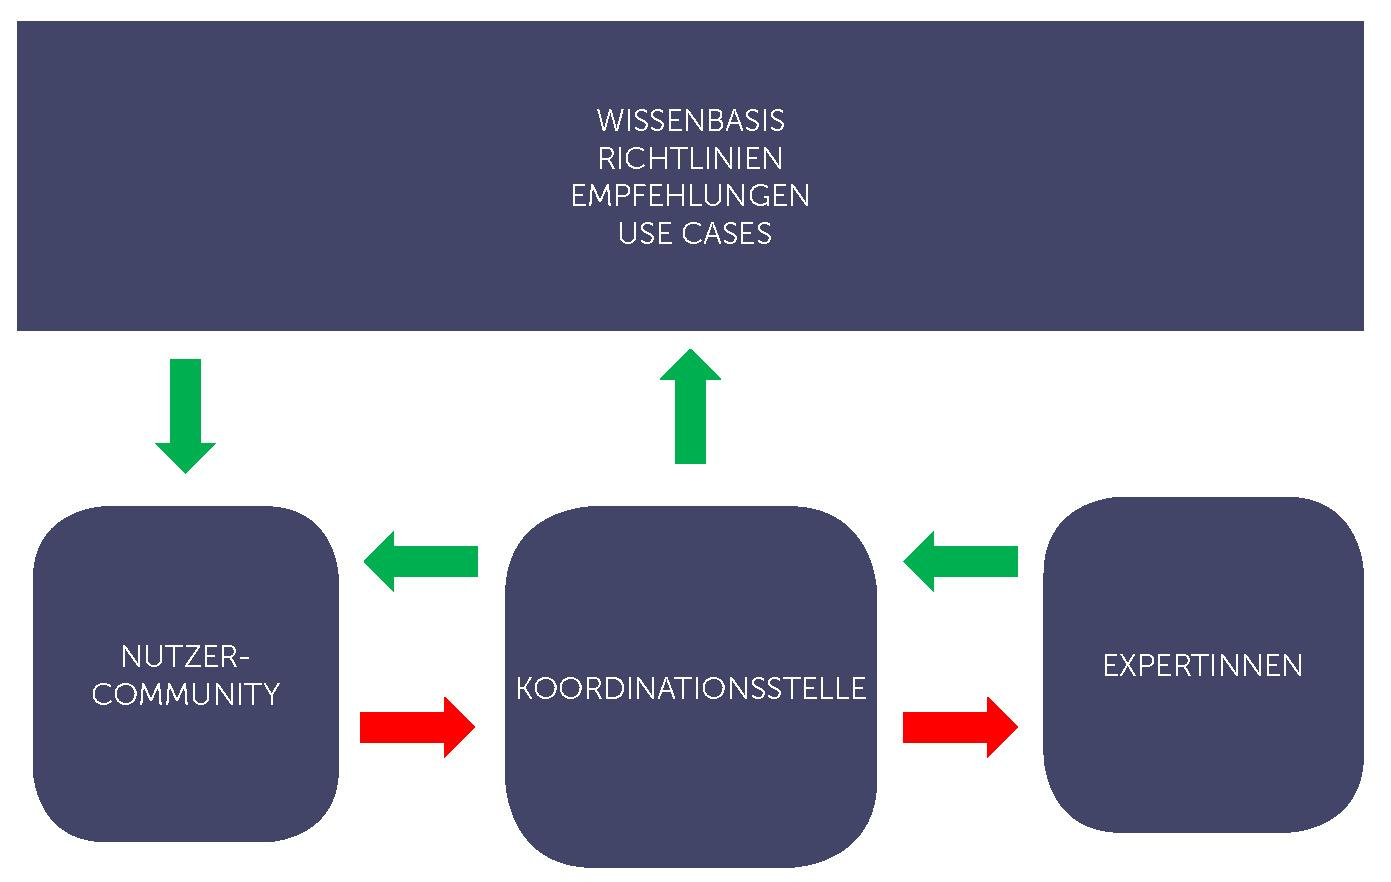
\includegraphics{img/Koordinationsstelle.jpg}
\caption{Die Rolle der Koordinationsstelle (Bild: Andrea Bertino, CC
BY-SA 4.0)}
\end{figure}

\hypertarget{diensteanbietersupport}{%
\subsection{Diensteanbieter/Support}\label{diensteanbietersupport}}

Wesentliche Teile der wissenschaftlichen Arbeit setzen die verlässliche
Zusammenarbeit zwischen verschiedenen AkteurInnen und Institutionen
voraus. Ohne diese Form der gegenseitigen freiwilligen Unterstützung
wäre die gute wissenschaftliche Praxis kaum zu gewährleisten -- man
denke etwa an Peer-Review-Verfahren für Aufsätze, wissenschaftliche
Gutachten und Projektanträge. Obwohl essenzielle Aktivitäten wie diese
selten monetär vergütet werden, sind sie für die jeweils Einzelnen doch
eine wichtige Quelle für wissenschaftliches Prestige und Anerkennung.
Ähnliches kann für Unterstützungsangebote für Dienste Virtueller
Infrastrukturen gelten, die NutzerInnen häufig die Möglichkeit geben,
fachspezifische Kenntnisse zu beweisen. Es wäre deshalb denkbar, die
Unterstützung des wissenschaftlichen Prozesses durch Angebote und die
dazugehörigen Supportleistungen in ähnlicher Weise zu honorieren. Dies
ist gleichwohl nur möglich, wenn sich die jeweiligen Diensteanbieter
öffentlich zur verbindlichen Betreuung der betreffenden Angebote und
Unterstützungsleistungen bereit erklären und konkrete
AnsprechpartnerInnen dafür zur Verfügung stellen. Transparenz der
Zuständigkeit und der verantwortlichen Kontaktpersonen ist die
grundlegende Prämisse dafür, dass der Mehrwert des jeweiligen Angebots
von der wissenschaftlichen Gemeinschaft wahrgenommen und entsprechend
wissenschaftlich honoriert werden kann.

\hypertarget{zentrale-koordinationsstelle}{%
\subsection{Zentrale
Koordinationsstelle}\label{zentrale-koordinationsstelle}}

\hypertarget{zusammensetzung-des-teams-kompetenzen}{%
\subsubsection{Zusammensetzung des Teams,
Kompetenzen}\label{zusammensetzung-des-teams-kompetenzen}}

Die zentrale Koordinationsstelle ist für die Verteilung der
verschiedenen Anfragen an die Kontaktpersonen der jeweiligen Angebote
zuständig. Sie umfasst ein beständiges Team an MitarbeiterInnen und
fungiert als fach- und angebotsübergreifender Bezugspunkt, der den
gesamten direkten Kommunikationsprozess mit der Community von der
Anfrage bis zur Beantwortung übernimmt. Die Mitglieder des Teams sollten
mit langfristigen Arbeitsverträgen ausgestattet sein, um die
Personalfluktuation und die damit verbundenen Aufwände für Einarbeitung
und Wissensaufbau zu reduzieren. Die Position erfordert ein Minimum an
technischer Kompetenz und eine profunde Kenntnis der gesamten
Infrastruktur, um eingehende Anfragen ohne Verzögerung den jeweils
zuständigen Kontaktpersonen zukommen lassen zu können.

\hypertarget{aufgabenspektrum}{%
\subsubsection{Aufgabenspektrum}\label{aufgabenspektrum}}

Da die Koordinationsstelle somit eine Schnittstelle zwischen NutzerInnen
und ExpertInnen bildet, muss jedes Mitglied mit dem gesamten Spektrum
der Infrastrukturangebote vertraut und dazu in der Lage sein,
NutzerInnen auch komplexe Lösungen für ihre Anfragen auf verständliche
Weise zu vermitteln. Der Koordinationsstelle obliegt ferner die Aufgabe,
die kommunizierten Lösungswege auch für Unbeteiligte nachvollziehbar und
transparent zu dokumentieren. Kommunikation ist demzufolge eines der
wichtigsten Aufgabenfelder der Koordinationsstelle und beinhaltet
insbesondere vier Elemente:

\begin{enumerate}
\def\labelenumi{\arabic{enumi}.}
\item
  die direkte Vermittlung zwischen NutzerInnen und ExpertInnen;
\item
  die interne Dokumentation der durchgeführten Beratungen inklusive der
  dazugehörigen Lösungen mitsamt aller Kommunikationsaktivitäten;
\item
  die darauf aufbauende Entwicklung von Materialien zur Unterstützung
  der NutzerInnen, unter anderem in Form von Informations- oder
  Schulungsunterlagen;
\item
  Aktivitäten, die darauf abzielen, in der Gemeinschaft der NutzerInnen
  ein klares Bewusstsein für den optimalen Arbeitsablauf der
  Supportanfragen selbst zu schaffen. Dabei muss durch geeignete
  Kommunikationsmaßnahmen sowohl auf den Webseiten der einzelnen
  Angebote als auch über verschiedene Informationskanäle klar
  kommuniziert werden, dass die erste Anlaufstelle für die Beantragung
  von Unterstützung für die einzelnen Angebote nicht die jeweils
  betreibende Institution ist, sondern die zentrale
  Koordinationsstelle.\footnote{Nichtsdestoweniger ist ebenfalls ein
    Verfahren notwendig, um direkt an Diensteanbieter gerichtete
    Anfragen regelmäßig an der zentralen Koordinationsstelle zu melden,
    um die Bearbeitungshistorie verfolgen, zentral dokumentieren und
    damit nachnutzen zu können.}
\end{enumerate}

Die Koordinationsstelle fungiert folglich als Bindeglied zwischen den
unterschiedlichen Leveln des Supports. Sie ist zunächst die zentrale
Anlaufstelle und übernimmt den First Level Support, indem sie eingehende
Anfragen in Form von Tickets zentral erfasst. Die Koordinationsstelle
sorgt sodann dafür, dass jede Anfrage die jeweils zuständigen
ExpertInnen des Second Level Supports erreicht und der gesamte
Beratungsprozess inklusive der erarbeiteten Lösungen dokumentiert wird.
Insofern liefert die Koordinationsstelle wichtige Impulse für den Third
Level Support, als sie basierend auf den dokumentierten Anfragen
gemeinsam mit dem Second Level Support Entwicklungsmöglichkeiten für die
Infrastruktur konzipiert und mit ExpertInnen der unterschiedlichen
Dienste diskutiert.

Im Einzelnen ergeben sich für die Koordinationsstelle daraus folgende
Aufgaben:

\begin{enumerate}
\def\labelenumi{\arabic{enumi}.}
\item
  Die Koordinationsstelle stellt sicher, dass der Kontakt mit den
  NutzerInnen aufrechterhalten wird und übernimmt die gesamte
  Kommunikation. Die Antwort auf die jeweilige Anfrage wird den
  NutzerInnen demzufolge NICHT von den für das Angebot zuständigen
  ExpertInnen übermittelt, sondern stattdessen von der
  Koordinationsstelle, welchedie Informationen bündelt und weiterleitet.
\item
  Die Koordinationsstelle gewährleistet, dass alle Schritte des
  Kommunikationsprozesses im Ticketsystem sowie zentral an einer anderen
  Stelle dokumentiert werden.
\item
  Die Koordinationsstelle prüft die dokumentierten Anfragen auf
  allgemeine Entwicklungen, fachspezifische Bedarfe, wiederkehrende
  Probleme, Weiterentwicklungsmöglichkeiten.
\item
  Die Koordinationsstelle lässt die aus den Anfragen gewonnenen
  Informationen den für die jeweiligen Angebote zuständigen
  Kontaktpersonen zukommen.
\item
  Die Koordinationsstelle formuliert gemeinsam mit den ExpertInnen des
  jeweiligen Angebots konkrete Maßnahmen zur Weiterentwicklung.
\end{enumerate}

\hypertarget{ausblick-nachhaltige-beratung-systematische-sicherung-von-wissen-gezielte-weiterentwicklung}{%
\section{Ausblick: Nachhaltige Beratung + systematische Sicherung
von Wissen = gezielte
Weiterentwicklung}\label{ausblick-nachhaltige-beratung-systematische-sicherung-von-wissen-gezielte-weiterentwicklung}}

Die aus der Einrichtung der Koordinationsstelle resultierende
Zentralisierung der Anfragen erlaubt einen Überblick über die Bedarfe
der Community von NutzerInnen. Dadurch wird es möglich, wiederkehrende
Probleme und Anfragen zu identifizieren und diese mit einschlägigen
Maßnahmen direkt zu adressieren. Hierzu können unter anderem
Informations-, aber auch Schulungsangebote zählen. Auf diese Weise lässt
sich nicht nur die Anzahl der Anfragen an den Helpdesk potentiell
reduzieren. Durch die auf dem Feedback der NutzerInnen basierende
Weiterentwicklung der Dienste und der dazugehörigen Informationsangebote
wird auch ein wichtiger Beitrag zur langfristigen Nutzbarkeit und damit
zur Nachhaltigkeit geleistet.

Um das reibungslose Zusammenspiel zwischen Koordinationsstelle,
Diensteanbietern und NutzerInnen zu gewährleisten und außerdem dafür zu
sorgen, dass das Feedback der NutzerInnen effektiv zur Entwicklung der
Angebote herangezogen wird, empfiehlt sich eine Gestaltung der
spezifischen Informationstätigkeit der Koordinationsstelle gemäß dem
folgenden Ablaufschema:

\begin{enumerate}
\def\labelenumi{\arabic{enumi}.}
\item
  Auf Grundlage der NutzerInnenanfragen werden Statistiken über die
  Angebote erstellt, für die sich eine Anpassung beziehungsweise
  Weiterentwicklung empfiehlt.
\item
  Ausgehend von diesen Statistiken legt die Koordinationsstelle eine
  Liste von Angeboten inklusive der dazugehörigen Prioritätsstufe vor,
  für die Bedarf an Weiterentwicklung bzw. Informationsmaterial besteht,
  etwa in Form von Updates, Funktionserweiterungen, Maßnahmen zur
  Dissemination, Schulungsunterlagen.
\item
  Diese Liste wird gemeinsam mit den AnsprechpartnerInnen der jeweiligen
  Dienste und weiteren ExpertInnen im Hinblick auf ihre
  Repräsentativität für die Bedürfnisse der NutzerInnen analysiert.
\item
  Auf Basis dieser Analyse wird ein erster Entwurf eines Entwicklungs-
  beziehungsweise Informationspapiers zum betreffenden Angebot
  konzipiert.
\item
  Nach gemeinsamer Prüfung durch alle Beteiligten wird das Dokument --
  beispielsweise als Factsheet -- auf der Website der digitalen
  Infrastruktur sowie in geeigneten Repositorien veröffentlicht.
\item
  Die zentrale Koordinationsstelle stellt darüber hinaus auch die
  Sichtbarkeit dieser Publikation über geeignete Social-Media-Kanäle
  sicher.
\item
  Am Ende eines jeden Jahres werden die verschiedenen
  Informationsdokumente in einer einzigen Veröffentlichung gesammelt und
  im Open Access sowie gegebenenfalls auch in gedruckter Form
  veröffentlicht.
\end{enumerate}

Ein auf diese Weise organisiertes System zur Weiterentwicklung und
Dissemination sorgt dafür, dass ein Helpdesk mehr leistet als bloßen
Support. Vielmehr trägt ein solcher Ansatz zur systematischen
Bedarfserhebung bei und wesentlich zu Aufbau, Anreicherung, Sicherung
und Dissemination des Wissens und leistet damit einen Beitrag zur
Nachhaltigkeit. Nur wenn neben der Kontinuität der Technik auch eine
Kontinuität des Wissens sichergestellt werden kann, ist die
Nachhaltigkeit digitaler Infrastrukturen nämlich erreichbar.

\hypertarget{literaturverzeichnis}{%
\section{Literaturverzeichnis}\label{literaturverzeichnis}}

Blümm, M., Neuroth, H. \& Schmunk, S. (2016). DARIAH-DE -- Architecture
of Participation. \emph{Bibliothek Forschung und Praxis}, 40(2),
pp.~165-171. \url{https://doi.org/10.1515/bfp-2016-0026}.

Busch, A., Meister, J. \& Schumacher, M. (2016). Wo bleibt eigentlich
der einzelne Fachwissenschaftler? \emph{Bibliothek Forschung und
Praxis}, 40(2), pp.~278-282.
\url{https://doi.org/10.1515/bfp-2016-0028}.

Gietz, P. \& Hütter, H. (2016). Der Aufbau einer nachhaltigen
technischen Infrastruktur für die Geisteswissenschaften: Die DARIAH-DE
eHumanities Infrastructure Service Unit (DeISU). \emph{Bibliothek
Forschung und Praxis}, 40(2), pp.
244-249.\url{https://doi.org/10.1515/bfp-2016-0029}.

Pufé, I. (2017). Nachhaltigkeit. 3., überarbeitete und erweiterte
Auflage. Konstanz/München: UVK (utb, 8705).

\hypertarget{abbildungsverzeichnis}{%
\section{Abbildungsverzeichnis}\label{abbildungsverzeichnis}}

Abb. 1: DARIAH-DE Entwicklung (Bild: Jan Rohden, CC-BY-SA 4.0)

Abb. 2: OTRS-System des DARIAH-DE Helpdesks (Screenshot:Andrea Bertino,
CC-BY-SA 4.0)

Abb. 3: Die Rolle der Koordinationsstelle (Bild: Andrea Bertino,
CC-BY-SA 4.0)

%autor
\begin{center}\rule{0.5\linewidth}{\linethickness}\end{center}

\textbf{Andrea Bertino} ist promovierter Philosoph und arbeitete mehrere
Jahre als wissenschaftlicher Mitarbeiter an den Universitäten Greifswald
und Regensburg. Seit 2017 ist er in den Abteilungen Elektronisches
Publizieren und Forschung und Entwicklung der Niedersächsischen Staats-
und Universitätsbibliothek Göttingen tätig, zunächst als Projektmanager
im EU-Project HIRMEOS und dann im DARIAH-DE Coordination Office.

\textbf{Jan Rohden } ist promovierter Romanist. In den vergangenen
Jahren war er zunächst Wissenschaftlicher Mitarbeiter an der
Universitäts- und Landesbibliothek Bonn, dann Fachreferent an der
Niedersächsischen Staats- und Universitätsbibliothek Göttingen. Seit
Dezember 2019 ist er in Geschäftsstelle der Max Weber Stiftung in Bonn
als Referent im Referat Forschungsdaten, Digital Humanities,
Bibliotheken tätig.

\end{document}
